\chapter{Preliminary Studies}
\label{chp:pre_study}

\noindent In this chapter, some preliminary studies of \gls{webrtc} business cases and prototype working scenario will be covered. The prototype working scenario is designed by considering different \gls{webrtc} usage cases.

\section{WebRTC Usage Cases}

\noindent In May 2011, Google released an open source project for browser-based real-time communication known as \gls{webrtc}. This has been followed by ongoing work to standardise the relevant protocols in the \gls{ietf} and browser \gls{api}s in the \gls{w3c}. Then more and more web application are using it in different ways. There are mainly two part of the \gls{webrtc} \gls{api}s could be used separately or cooperatively in the different web application.

\begin{itemize}[topsep=-1em,parsep=0em,itemsep=0em]
 \item \textbf{MediaStream:} get access to data streams, such as from the user's camera and microphone.
 \item \textbf{RTCPeerConnection:} audio or video calling, with facilities for encryption and bandwidth management.
 \item \textbf{RTCDataChannel:} peer-to-peer communication of generic data.
\end{itemize}

\par Because most of the application need to get the user's camera view and microphone sound, the \textit{MediaStream} \gls{api} is used always in real-time communication application. Normally \textit{MediaStream} \gls{api} will be used along with \textit{RTCPeerConnection} for showing remote peer media source content. The following business usage cases, 'Tropo' and 'Uberconference', are in this category.

\subsection{Tropo}

\par Tropo is an application platform that enables web developers to write communication applications in the languages they already use, Groovy\footnote{Groovy is an object-oriented programming language for the Java platform. It is a dynamic language with features similar to those of Python, Ruby, Perl, and Smalltalk.\cite{wiki:groovy}}, Ruby\footnote{Ruby is a dynamic, reflective, object-oriented, general-purpose programming language. It was designed and developed in the mid-1990s by Yukihiro "Matz" Matsumoto in Japan.\cite{wiki:ruby}}, \gls{php}\footnote{PHP is a server-side scripting language designed for web development but also used as a general-purpose programming language.\cite{wiki:php}}, Python\footnote{Python is a widely used general-purpose, high-level programming language.\cite{wiki:python}} and JavaScript\footnote{JavaScript (JS) is a dynamic computer programming language.\cite{wiki:js}}, or use a Web \gls{api} which will talk with an application running on your own server through the use of \gls{http} and \gls{json}, feeding requests and processing responses back and forth as needed. Tropo is in the cloud, so it manages the headaches of dealing with infrastructure and keeping applications up and running at enterprise-grade. With Tropo, developers can build and deploy voice and telephony applications, or add voice to existing applications.\cite{web:tropo}

\par It has some advanced features, like 'Phone numbers around the world', 'Text messaging', 'Transcription', 'Call Recording', 'Conferencing', 'Text to Speech' and 'Speech Recognition'. The prototype system in this thesis will provide similar functions like 'Text messaging' and 'Conferencing'. Since Tropo is a cloud application platform, it generates its own scripts based on programming language to provide developer possibility to easily use \gls{webrtc} to communicate with other kinds of network rather than \gls{ip} network. The functions Tropo provided is implemented in application server in the prototype, the application server will handle both the \gls{sip} stack and \gls{webrtc} stack in the system. For the client scripts will be host on the same application server for browser user to access and use.

\subsection{Uberconference}

\par UberConference fixes all the broken and outdated aspects of traditional conference calling, making it a more productive business tool, and transforming an industry that hasn't seen real innovation in decades. UberConference gives a visual interface to every conference call so callers can know who's on a call and who's speaking at any time, in addition to making many other features, such as Hangouts\footnote{Google Hangouts is an instant messaging and video chat platform developed by Google, which launched on May 15, 2013 during the keynote of its I/O development conference.\cite{wiki:hangouts}} integration and screen sharing, easy-to-use with the click of a button. Built by the teams that brought Google Voice\footnote{Google Voice (formerly GrandCentral) is a telecommunications service by Google launched on March 11, 2009.\cite{wiki:googleVoice}} and Yahoo! Voice to tens of millions of users, UberConference launched in 2012 and is funded by Andreessen Horowitz and Google Ventures.\cite{web:uberconference}

\begin{wrapfigure}{r}{0.6\textwidth}
	\centering
    	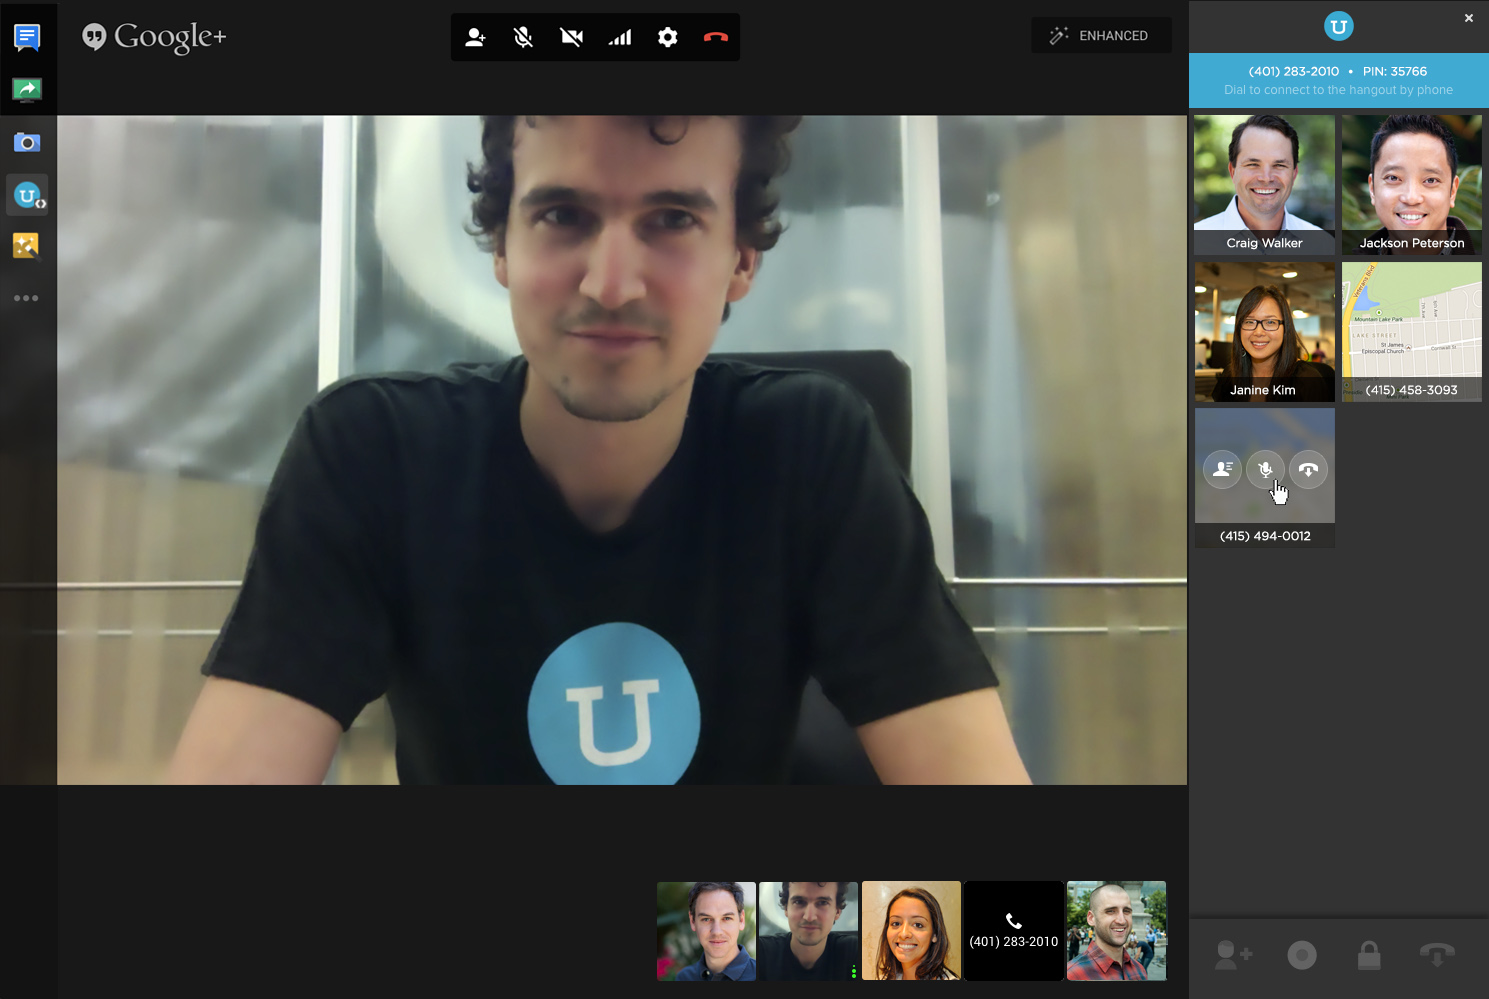
\includegraphics[width=0.58\textwidth,natwidth=610,natheight=642]{figs/uberconference_hangout.jpg}
  	\caption{UberConference integrate with Hangouts Screen shot\cite{tnw:uberconference}}
  	\label{fig:uberconference}
\end{wrapfigure}

\par The prototype system in this thesis is ideally to provide same rich media communication platform as the service provided by UberConference. In February of 2014, UberConference release the new feature which allow user to call into a Google Hangouts session with their mobile phone. The feature is shown in Figure \ref{fig:uberconference}, Once you have installed the UberConference app in Hangouts, people can join your call via phone with the help of a dedicated number. The prototype system will provide the same real-time communication service, but allow the user to create a video conference based on \gls{webrtc} on browser by their mobile phone number and communicate with audio only mobile phone user as well. It will be more easier for user since they just need to remember their user credential related to their mobile phone number in order to use the prototype application rather than register another service user binding with private telephone number. During the real-time conversation, the prototype application will provide user cooperation tools like instance message and file sharing in this development phase.

\subsection{Cube Slam}

\noindent However, there is another important \gls{api}, \textit{RTCDataChannel} , can be used more creatively by the developer to build web applications. The experiment  usage cases, 'Cube Slam' and 'Webtorrent', are in this category which is using \textit{RTCDataChannel} to build \gls{p2p} data sharing without data going though the server to dispatch to other peers. It works more efficiently to handle the synchronization problem.

\par Cube Slam (shown in Figure \ref{fig:cube_slam}) is a Chrome Experiment built with \gls{webrtc} , play an old-school arcade game with your friends without downloading and installing any plug-ins. Cube Slam uses \textit{getUserMedia} to access user's webcam and microphone ,\textit{RTCPeerConnection} to stream user video to another user, and \textit{RTCDataChannel} to transfer the bits that keep the gameplay in sync. If two users are behind firewalls, \textit{RTCPeerConnection} uses a TURN  relay server (hosted on Google Compute Engine) to make the connection. However, when there are no firewalls in the way, the entire game happens directly peer-to-peer, reducing latency for players and server costs for developers.\cite{chrome:cube_slam}

\begin{figure}
	\centering
    	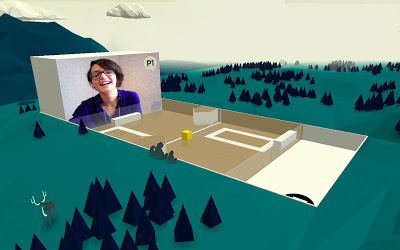
\includegraphics[width=0.8\textwidth,natwidth=610,natheight=642]{figs/cube_slam.jpg}
  	\caption{Cube Slam Game Over Screen}
  	\label{fig:cube_slam}
\end{figure}

\par The idea behind the Cube Slam is that use \textit{RTCDataChannel} to sync the player data in real-time to reduce the latency by peer to peer. \textit{RTCDataChannel} sends data securely, and supports an "unreliable" mode for cases where you want high performance but don't care about every single packet making it across the network. In cases like games where low delay often matters more than perfect delivery, this ensures that a single stray packet doesn't slow down the whole app. The prototype application in this thesis will still use WebSocket for data sharing instead of \textit{RTCDataChannel} because the media server using in this system is not support \textit{RTCDataChannel} yet, so it is not possible to create peer to peer session regarding to this issue. This case about using \textit{RTCDataChannel} in prototype application will be discussed in Chapter \ref{chp:future_work}.

\subsection{Webtorrent}

\par The goal of project Webtorrent is to build a browser BitTorrent client that requires no install, no plugin, no extension, and fully-interoperates with the regular BitTorrent network. It uses \gls{webrtc} Data Channels for peer-to-peer transport. Since WebTorrent is web-first, it's simple for users who do not understand .torrent files, magnet links, NATs, etc. By making BitTorrent easier, it will be accessible to new swathes of users who were previously intimidated, confused, or unwilling to install a program on their machine to participate.\cite{github:webtorrent}

\par Since \gls{webrtc} is usually used for peer to peer communication, the \textit{RTCDataChannel} can be used in more creative way like Webtorrent. Although it need to keep the browser up and running on both ends, then there will be no asynchronous nature into it, it does reduce the bandwidth required and it adds privacy as to who has access to the file being shared. Since the application can reach direct between browsers, it can use the data channel to create a low latency network, where data is shared directly without going through servers on the way. It is lower cost for the developer and more secure on this case. For example, doing the same using a drastically larger number of web browser nodes as \gls{tor}\footnote{Tor (previously an acronym for The Onion Router) is free software for enabling online anonymity and censorship resistance. Tor directs Internet traffic through a free, worldwide, volunteer network consisting of more than five thousand relays to conceal a user's location or usage from anyone conducting network surveillance or traffic analysis.\cite{wiki:tor}}, increases the chance of privacy.This can reduce the need for “real” web servers to run services, and use those only as points of access into the dynamic network that is created ad-hoc.

\section{Prototype Working Scenario}

\noindent The prototype system in this thesis will pay more attention on the real-time communication usage of \gls{webrtc}. The main purpose of the system is to combine internet browser user and traditional telephony user without complicate instillation, plugin and extension. There are two typical working scenarios of the prototype system will be described below.

\subsection{Advanced 'one-number' communication platform}

\par Adam is a typical Facebook\footnote{Facebook is an online social networking service.} user and he does synchronize his contact list through Google Contacts\footnote{Google Contacts is Google's contact management tool that is available in its free email service Gmail, as a standalone service, and as a part of Google's business-oriented suite of web apps Google Apps.\cite{wiki:google_contacts}} by his smart phone. Now his operator provides user credential from his telephone number to him. Then Adam just login on his operator 'FellowPhone' web page, now he can import his contacts list through his Google contact list. After that, he can see if his contact person is online by using the same web application 'FellowPhone' or not. He can also import his Facebook friends list and fulfill the friends list with his contacts list information. Therefore, Adam can see if his facebook friends online or not. If his facebook friends/ Google contacts are online and use 'FellowPhone' web application from their operator, Adam can invite them have a video conference otherwise his friends are not online then he can still invite them into the video conference but though his friends mobile phone with only audio sound.

\par During the video conference, Adam can send his online friends files and instance messages (website links, video links and so on). Moreover, his offline friends in the same conference will get the same information as text \gls{sms}. Adam can reach his friends wherever they are and no matter if they are online or not as long as they have their mobile phone. 

\subsection{Multiple doctors consultation room}

\par Eve is a 80-year-old lady, she lives with her children in their house. But at the day time, her children go to work, she need take care of herself. She has appointment with her doctor about her backache. But she can not go to hospital or family doctor office. Then she use her mobile phone to call her family doctor. Her family doctor, Isak using the prototype service from his company and operator. When Eve call to her doctor, Isak, for help, Isak answered her phone and try to get her previous medical information from other system. Then he found out that Eve had other doctor about her back treatment before. He can just login in the prototype system and find out if the other doctor is at work (online in the system). The other doctor, Stella, she has the treatment log about Eve. She got invitation to join the current conversion with Isak and Eve. She can send message to Isak and share the treatment log with Isak if necessary. She can listen to the talk between Isak and Eve about the new update of the treatment to give suggestion. Isak can ask for more different doctors in the system for advice and consultation to help Eve case.

\par But in Eve aspect, she only calls doctor Isak, and she can got help from more than one doctor at the same time. If it is necessary, she can use the computer to login the same system to have video conference with different doctors for her case. The only thing required for her is a telephone number and a mobile phone.